 
% This is "sig-alternate.tex" V2.0 May 2012
% This file should be compiled with V2.5 of "sig-alternate.cls" May 2012
%
% This example file demonstrates the use of the 'sig-alternate.cls'
% V2.5 LaTeX2e document class file. It is for those submitting
% articles to ACM Conference Proceedings WHO DO NOT WISH TO
% STRICTLY ADHERE TO THE SIGS (PUBS-BOARD-ENDORSED) STYLE.
% The 'sig-alternate.cls' file will produce a similar-looking,
% albeit, 'tighter' paper resulting in, invariably, fewer pages.
%
% ----------------------------------------------------------------------------------------------------------------
% This .tex file (and associated .cls V2.5) produces:
%       1) The Permission Statement
%       2) The Conference (location) Info information
%       3) The Copyright Line with ACM data
%       4) NO page numbers
%
% as against the acm_proc_article-sp.cls file which
% DOES NOT produce 1) thru' 3) above.
%
% Using 'sig-alternate.cls' you have control, however, from within
% the source .tex file, over both the CopyrightYear
% (defaulted to 200X) and the ACM Copyright Data
% (defaulted to X-XXXXX-XX-X/XX/XX).
% e.g.
% \CopyrightYear{2007} will cause 2007 to appear in the copyright line.
% \crdata{0-12345-67-8/90/12} will cause 0-12345-67-8/90/12 to appear in the copyright line.
%
% ---------------------------------------------------------------------------------------------------------------
% This .tex source is an example which *does* use
% the .bib file (from which the .bbl file % is produced).
% REMEMBER HOWEVER: After having produced the .bbl file,
% and prior to final submission, you *NEED* to 'insert'
% your .bbl file into your source .tex file so as to provide
% ONE 'self-contained' source file.
%
% ================= IF YOU HAVE QUESTIONS =======================
% Questions regarding the SIGS styles, SIGS policies and
% procedures, Conferences etc. should be sent to
% Adrienne Griscti (griscti@acm.org)
%
% Technical questions _only_ to
% Gerald Murray (murray@hq.acm.org)
% ===============================================================
%
% For tracking purposes - this is V2.0 - May 2012

\documentclass{sig-alternate}

%%%%%%%%%%%%%%%%%%%%%%%%%%%%%%%%%%%%%%%%%%%%%%%%%%%
%%%%%Imports%%%%%%%%%%%%%%%%%%%%%%%%%%%%%%%%%%%%%%%
%%%%%%%%%%%%%%%%%%%%%%%%%%%%%%%%%%%%%%%%%%%%%%%%%%%

\usepackage[mathletters]{ucs}
\usepackage{amssymb}
\usepackage[utf8x]{inputenc}
\usepackage[cyr]{aeguill}
\usepackage[english]{babel}
\usepackage{fancyhdr, ifpdf}
\usepackage{array}
\usepackage{multirow}
\usepackage{textcomp}
\usepackage{verbatim} 
\usepackage{listings}
\usepackage{hyperref}
\usepackage{dsfont}
\usepackage{fontspec}
\usepackage{booktabs}
\usepackage{amsmath,amssymb,amstext,mathtext}
\usepackage{tabularx}
\usepackage{longtable}
\usepackage{url}
\usepackage{spverbatim}
\usepackage{changepage}
\usepackage{caption}
\usepackage{subcaption}

\makeatletter
\def\url@leostyle{%
  \@ifundefined{selectfont}{\def\UrlFont{\sf}}{\def\UrlFont{\small\ttfamily}}}
\makeatother

\newcommand{\loadencoding}[1]{%
  \begingroup
  \def\DeclareUnicodeCharacter##1##2{%
    \expandafter\gdef\csname uni\number"##1\endcsname
      {{\fontencoding{#1}\selectfont##2}}}
  \makeatletter
  \lowercase{\input{#1enc.dfu}}%
  \endgroup}
\newcommand\unisymbol[1]{\csname uni\number#1\endcsname}
\loadencoding{T1}
\loadencoding{T2A}
\newfontfamily\unicodefont{Arial Unicode MS}
\newfontfamily\codefont{Courier}


\begin{document}
%
% --- Author Metadata here ---
\conferenceinfo{Joint Conference on Digital Libraries}{2015 Knoxville, USA}
%\CopyrightYear{2007} % Allows default copyright year (20XX) to be over-ridden - IF NEED BE.
%\crdata{0-12345-67-8/90/01}  % Allows default copyright data (0-89791-88-6/97/05) to be over-ridden - IF NEED BE.
% --- End of Author Metadata ---

\title{  {\Huge $ \ttlfnt{5e^{x+y}}$}: Searching over mathematical content in digital libraries}

%
% You need the command \numberofauthors to handle the 'placement
% and alignment' of the authors beneath the title.
%
% For aesthetic reasons, we recommend 'three authors at a time'
% i.e. three 'name/affiliation blocks' be placed beneath the title.
%
% NOTE: You are NOT restricted in how many 'rows' of
% "name/affiliations" may appear. We just ask that you restrict
% the number of 'columns' to three.
%
% Because of the available 'opening page real-estate'
% we ask you to refrain from putting more than six authors
% (two rows with three columns) beneath the article title.
% More than six makes the first-page appear very cluttered indeed.
%
% Use the \alignauthor commands to handle the names
% and affiliations for an 'aesthetic maximum' of six authors.
% Add names, affiliations, addresses for
% the seventh etc. author(s) as the argument for the
% \additionalauthors command.
% These 'additional authors' will be output/set for you
% without further effort on your part as the last section in
% the body of your article BEFORE References or any Appendices.

\numberofauthors{3} %  in this sample file, there are a *total*
% of EIGHT authors. SIX appear on the 'first-page' (for formatting
% reasons) and the remaining two appear in the \additionalauthors section.
%
% You can go ahead and credit any number of authors here,
% e.g. one 'row of three' or two rows (consisting of one row of three
% and a second row of one, two or three).
%
% The command \alignauthor (no curly braces needed) should
% precede each author name, affiliation/snail-mail address and
% e-mail address. Additionally, tag each line of
% affiliation/address with \affaddr, and tag the
% e-mail address with \email.
%
% 1st. author
\author{
\alignauthor Arthur Oviedo\\
  \affaddr{EPFL, Switzerland.}\\%
  \affaddr{arthur.oviedo@alumini.epfl.ch}%
\alignauthor Nikos Kasioumis \\
  \affaddr{CERN, Switzerland.}\\%
  \affaddr{nikos.kasioumis@cern.ch}%
\alignauthor Karl Aberer\\%
  \affaddr{EPFL, Switzerland.}\\%
  \affaddr{karl.aberer@epfl.ch}%
}

\maketitle
\begin{abstract}
This paper presents $5e^{x+y}$, a system that is able to extract, index and query mathematical content expressed as mathematical equations, complementing the CERN Document Server (CDS)\cite{CDS1}. We present the most important aspects of its design, our approach to model the relevant features of the mathematical content, and provide a demonstration of its searching capabilities.

\end{abstract}

\section{Introduction}
CDS (CERN Document Server) is the institutional digital repository developed and used at CERN\cite{CERN}. It contains more than 1,000,000 records and stores more than 400,000 full text documents, organized in different collections among published articles, books and preprints. Invenio\cite{invenio} is the open-source digital library software platform behind CDS and it is developed in parallel to CDS at CERN. Besides CDS, Invenio supports around thirty scientific institutions worldwide including INSPIRE (a collaboration between Fermilab, CERN, DESY and SLAC) EPFL and ILO. 
A considerable amount of the full text documents on CDS contain mathematical content, represented in the form of equations. The Preprints collection alone contains more than 700,000 records, harvesting documents from services like ArXiV\cite{arxiv} where most of the documents are in the areas of physics, mathematics and statistics which are very rich in this type of content. Even though Invenio provides a powerful search engine that allows users to query records using different fields like author or keywords, it is not suitable for mathematical content. $5e^{x+y}$ is developed as a first attempt to address this limitation by allowing querying for records based on mathematical equations.

\section{System Overview}
In this section we provide a general overview of the main design points of $5e^{x+y}$. A more detailed description of the system can be found in \cite{mathexplorerweb}.

\subsection{Features Extraction}
Our initial focus in the project was to define a good set of features that we could extract and index from our equations. We divide them into two different categories: notational and structural features. The notational features relate to the actual naming and representation of the different elements of the equation. The selected format for representation and internal processing of the equations was MathML. This language allows for easier processing because of its markup nature and has a stronger support from the W3C among other communities. For the notational features we extract the leaf elements of the equation: variables, numbers and operators represented by the <mi>, <mn> and <mo> tags respectively. In addition, we index 2-grams and 3-grams of symbol-operator and symbol-operator-symbol sequences.

We perform some processing of these tokens such as normalizing and decomposing of complex characters. This allows us to partially match characters with different unicode points but similar or equal visual rendering. For instance LATIN CAPITAL LETTER A WITH RING ABOVE with code 0xc5 and ANGSTROM SIGN with code 0x212b both are rendered as \r{A} and can both be used to refer to the Angstrom measurement unit. Following this example, we index both the original token <mi>\r{A}</mi> and the normalized form <mi>\r{A}</mi> <mi>A</mi>.For operators which are semantically related such as comparison, integrals and arithmetic, we apply another set of rules since their unicode characters do not provide an easy way to match them.
For example the INTEGRAL character with code 0x222b generates the tokens <mo>{\unicodefont ∫}</mo> and INT\_OP and the CONTOUR INTEGRAL character with code 0x222e generates the tokens <mo>{\unicodefont ∮} </mo> and INT\_OP. In this way, both have a partial matching in the second token.

The second set of features relate to the structure of the equation. Two different properties of mathematical equations impose additional challenges for a Mathematics Information Retrieval (MIR) system. First, variables can be used indistinguishably and any character set can be used to represent the same equation. For example, $f(t) = vt + c $ and $g(x) = ac + b$ can represent the same linear equation, however the context in which each variable is used follows certain conventions. To address this issue, we relied on pattern matching, a very powerful feature that current Computer Algebra Systems (CAS) provide. We integrated Mathematica\cite{mathematica} into our system, to perform pattern matching on the equations and identify occurrences within a predefined set of patterns. This allows us to detect if the equation contains certain types of common algebraic structures. For instance, the pattern {\codefont a\_.x\^{} 2 + b\_.x + c\_.} is used to identify a quadratic expression. This mechanism is very powerful since \_.x represents any type of expression, not only a single term. 

An additional challenge mathematical equations pose is the fact that a given equality can be rewritten in multiple ways taking into account properties of the different operators like associativity, distributivity and commutativity among others. Our approach relies once more in the features provided by Mathematica: we perform the {\codefont Simplify} operation which applies a set of predefined rules on a given equation with the goal of providing a canonical representation.

\subsection{System architecture}
$5e^{x+y}$ is implemented on top of the Lucene/Solr \cite{solr} framework. We expanded the default schema with several fields, the most important ones being: the {\codefont math\_notational\_field} which stores all the described tokens and n-grams, \\ the {\codefont math\_structural\_field} which stores the occurrences of predefined algebraic structures and the {\codefont filename} which is used to store the file/record where the particular equation was found. 

In order to extend Lucene with the new use case, our work extends some of the base classes. {\codefont MultiplePatternTokenizer} is in charge of producing a stream of tokens from a single equation. These tokens are identified by applying multiple regular expressions. {\codefont UnicodeNormalizingFilter} applies the unicode normalizing transformation described above. {\codefont SynonymExpandingFilter} expands operators, using a manually computed table based on \cite{math_groups}, with the category they belong to. Finally {\codefont StructuralPatternsTokenizer} provides the pattern matching functionality by establishing communication with Mathematica's {\codefont Kernel Link} API.

To integrate $5e^{x+y}$ with Invenio, we used the {\codefont solrpy} library which communicates with an instance of Solr running $5e^{x+y}$ as a plugin. Since Solr provides different integrating mechanisms with external systems, $5e^{x+y}$ can be easily be incorporated into different digital libraries.

\section{Demonstration}
As part of the demonstration of $5e^{x+y}$, we present a demo instance of the Invenio software with the mathematical equations search functionality.
The user can access the mathematical search functionality through a link in the main page. Once there, the user is presented with a classic search functionality where they can input an equation. The equation can be expressed in either \LaTeX or MathML. To ease the writing of \LaTeX code, we include an online editor\cite{latex_editor} that renders the input as the user types it. \LaTeX code is usually more familiar to users, however, the internal representation is in MathML as previously explained. The translation from \LaTeX to MathML is done through the third party library SnuggleTex\cite{snuggletex} that has some shortcomings, so we allow users to input the query in MathML as well. When the query is ready, the user can click the submit button and the system then performs the search. Once the system has performed the lookup and produced the results, they are presented to the user.
The system displays the 20 results with the highest score. Each result shows the matched equation snippet, the title of the record containing the given equation and the link to the record.

%\begin{figure}
%\center
%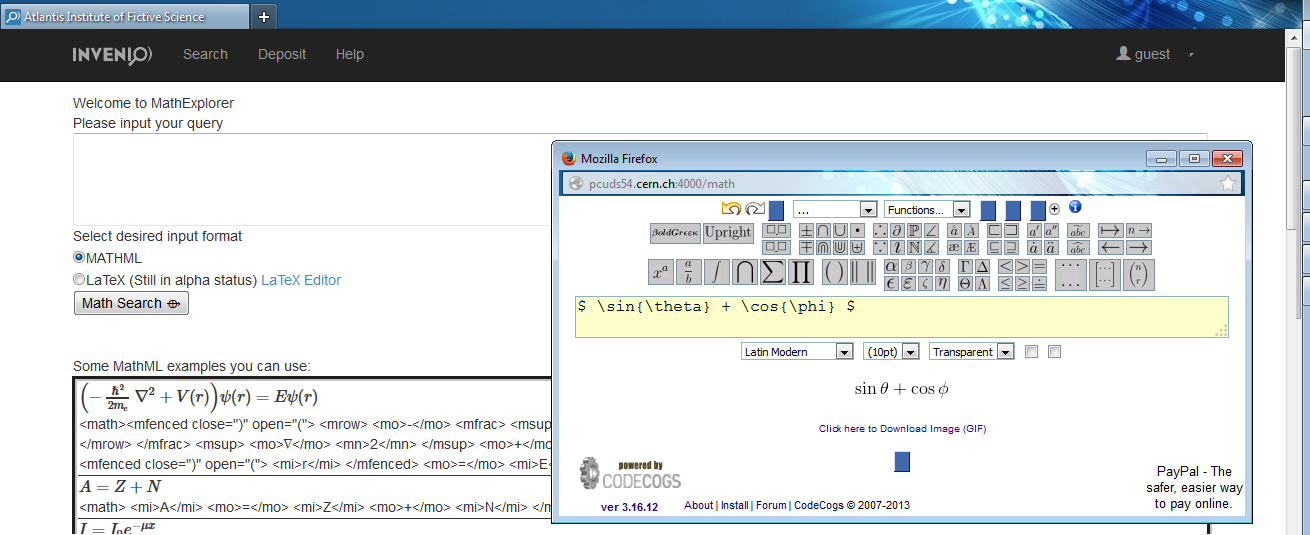
\includegraphics[height=3 cm]{images/figures/input_interface.png}
%\label{input_int}
%\caption{Web interface of $5e^{x+y}$: Query input screen}
%\end{figure}
%
%\begin{figure}
%\center
%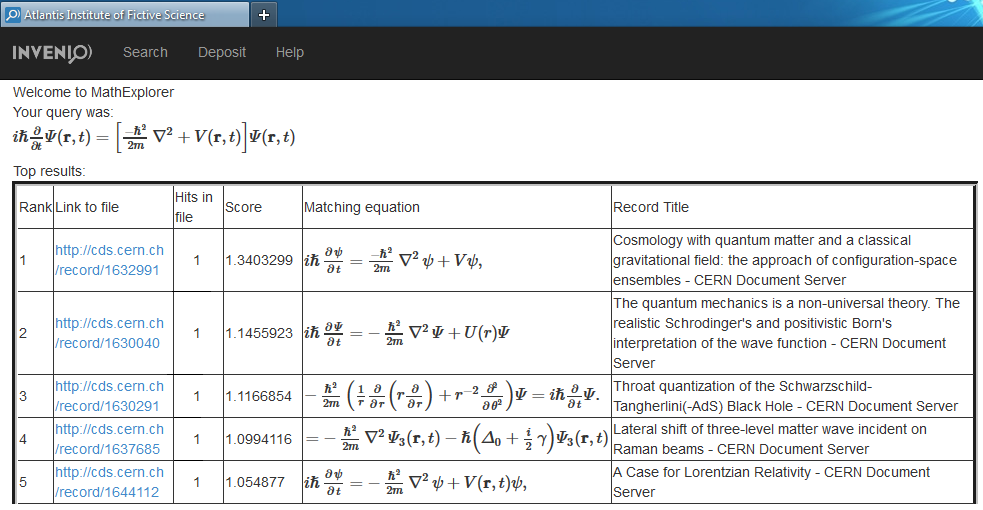
\includegraphics[height=3 cm]{images/figures/results_interface.png}
%\label{results_int}
%\caption{Web interface of $5e^{x+y}$: Results screen}
%\end{figure}

\begin{figure}
\centering
\begin{minipage}{.27\textwidth}
  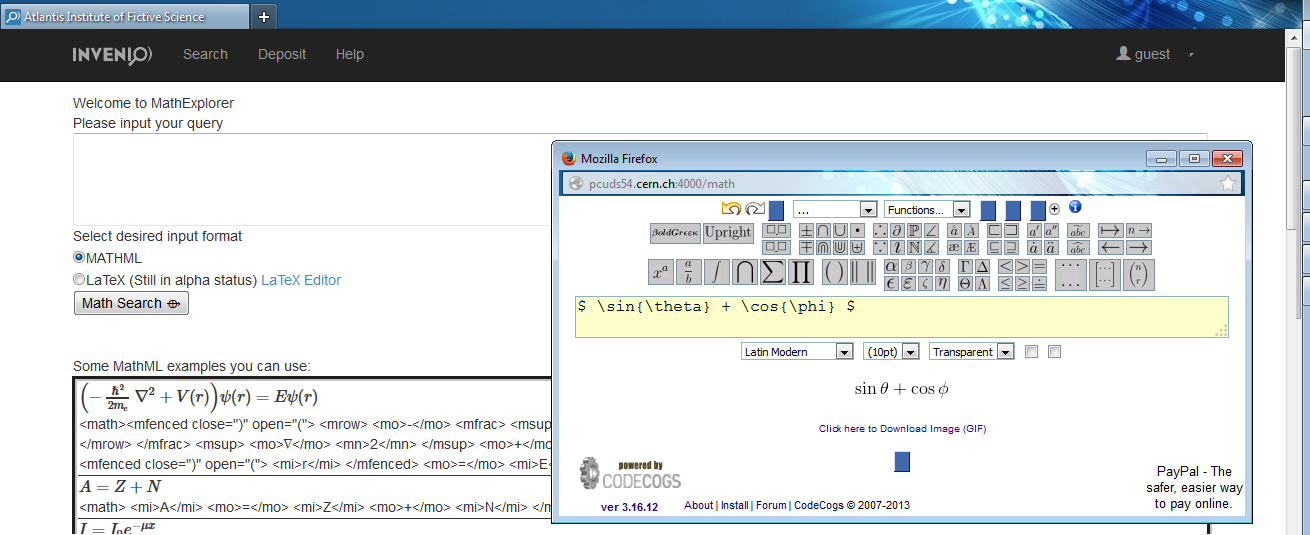
\includegraphics[width=0.9\linewidth]{images/figures/input_interface.png}
  \captionof{figure}{Input interface.}
  \label{fig:test1}
\end{minipage}%
\begin{minipage}{.27\textwidth}
  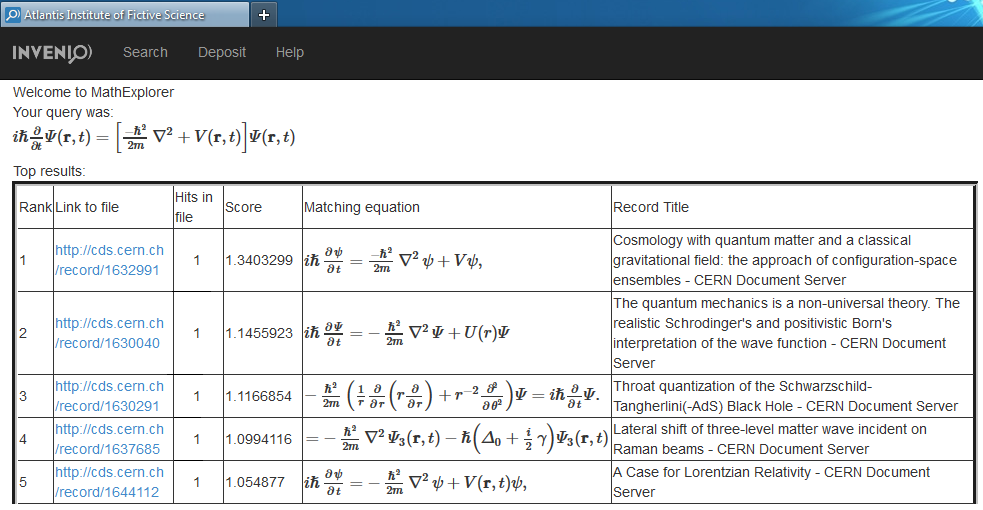
\includegraphics[width=0.9\linewidth]{images/figures/results_interface.png}
  \captionof{figure}{Result page.}
  \label{fig:test2}
\end{minipage}
\end{figure}

\section{Conclusions}

In this demonstration, we presented an important limitation of CDS, and how our system, $5e^{x+y}$, provides efficient and precise searching capabilities over mathematical to our system. We presented our approach to model mathematical equations in terms of two different types of features. How we extended the Lucene/Solr Framework to handle our specific type of content and how through the Mathematica CAS, we were able to include powerful functionalities such as pattern matching and equation simplificiation to our system, and use them to improve the quality of the results. Finally we presented our integration mechanism with the Invenio software through the solarpy library.

\section{Availability}
Both the Invenio software and the $5e^{x+y}$ module are open-source software available through GPL Licence. Invenio can be downloaded from \url{http://invenio-software.org/}. $5e^{x+y}$ can be downloaded from \\ \url{https://github.com/arthoviedo/cern_math_explorer}. 

%ACKNOWLEDGMENTS are optional
%
% The following two commands are all you need in the
% initial runs of your .tex file to
% produce the bibliography for the citations in your paper.
\bibliographystyle{abbrv}
\bibliography{bibliography}  % sigproc.bib is the name of the Bibliography in this case
% You must have a proper ".bib" file
%  and remember to run:
% latex bibtex latex latex
% to resolve all references
%
% ACM needs 'a single self-contained file'!
%
%APPENDICES are optional
%\balancecolumns
\end{document}
